\documentclass{beamer}
\usepackage{relsize}
\usepackage{color}

\usepackage{listings}
\usetheme{CambridgeUS}
%\usepackage{beamerthemesplit} % new
\usepackage{enumitem}
\usepackage{amsmath}                    % See geometry.pdf to learn the layout options.
\usepackage{amsthm}                   % See geometry.pdf to learn the layout options. There
\usepackage{amssymb}                    % See geometry.pdf to learn the layout options.
\usepackage[utf8]{inputenc}
\usepackage{graphicx}
\usepackage[english,bulgarian]{babel}

\lstset{language=C++,
                basicstyle=\ttfamily,
                keywordstyle=\color{blue}\ttfamily,
                stringstyle=\color{red}\ttfamily,
                commentstyle=\color{green}\ttfamily,
                morecomment=[l][\color{magenta}]{\#}
}

\newtheorem{mydef}{Дефиниция}[section]
\newtheorem{lem}{Лема}[section]
\newtheorem{thm}{Твърдение}[section]

\DeclareMathOperator{\restrict}{\upharpoonright}

\setitemize{label=\usebeamerfont*{itemize item}%
  \usebeamercolor[fg]{itemize item}
  \usebeamertemplate{itemize item}}

\setbeamercovered{transparent}



\begin{document}
\title[Структури от данни и програмиране]{Балансирани дървета}
\author{Калин Георгиев}
\frame{\titlepage}

\section{Ротации}

\begin{frame}[fragile]
\frametitle{Прости ротации}

\begin{itemize}
  \item Балансиращ фактор, $bf(r)=h(r.right)-h(r.left)$
\end{itemize}

\begin{columns}[t]
  \begin{column}{0.5\textwidth}
      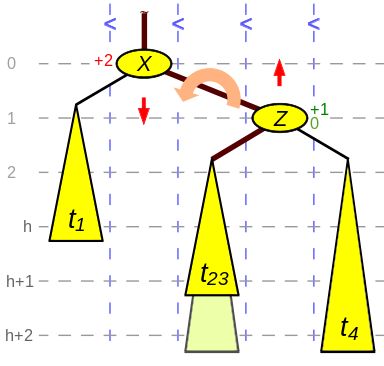
\includegraphics[width=4.5cm]{images/bal_tree_left_rotation_1}
  \end{column}
  \begin{column}{0.5\textwidth}
       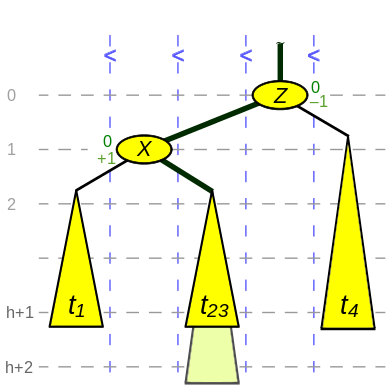
\includegraphics[width=4.5cm]{images/bal_tree_left_rotation_2}
  \end{column}
\end{columns}
\centerline{Лява ротация[1]}

\end{frame}


\begin{frame}[fragile]
  \frametitle{Двукратни ротации}
    
  \begin{columns}[t]
    \begin{column}{0.33\textwidth}
        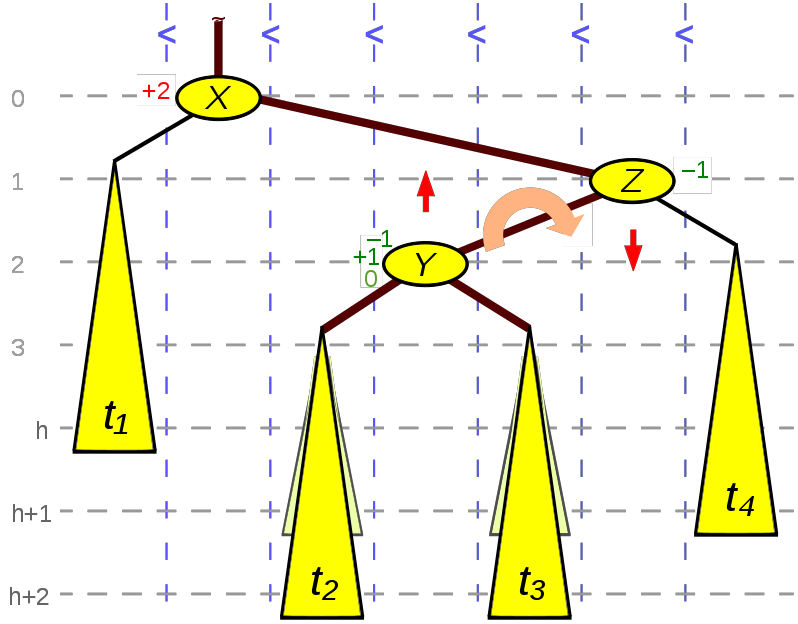
\includegraphics[width=4cm]{images/bal_tree_right_left_rotation_1}
    \end{column}
    \begin{column}{0.33\textwidth}
         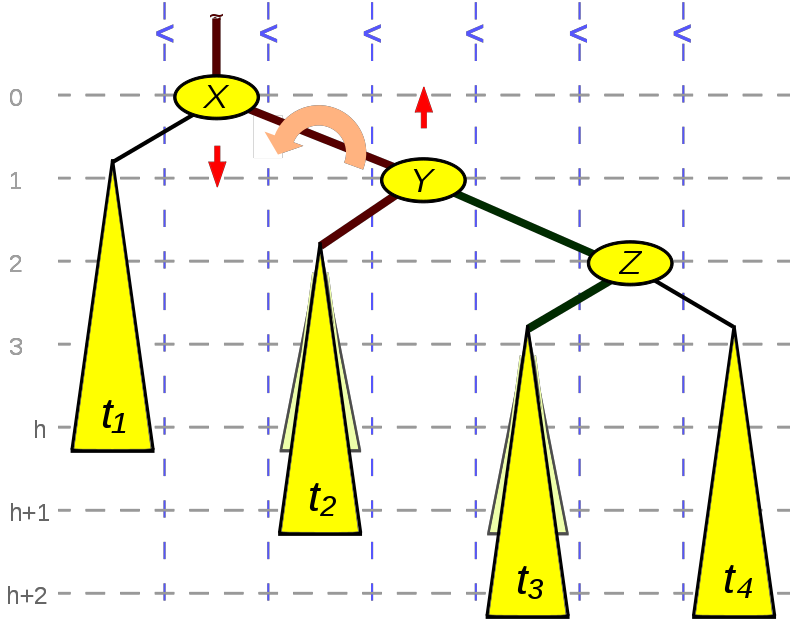
\includegraphics[width=4cm]{images/bal_tree_right_left_rotation_2}
    \end{column}
    \begin{column}{0.33\textwidth}
      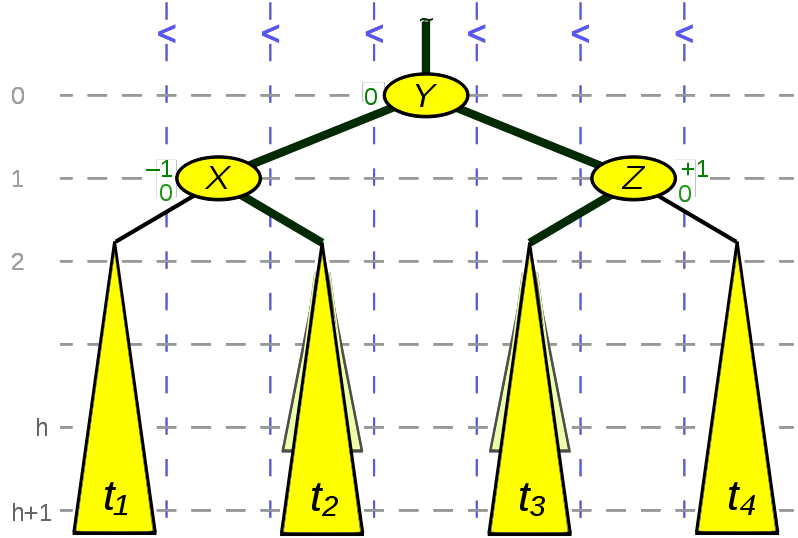
\includegraphics[width=4cm]{images/bal_tree_right_left_rotation_3}
 \end{column}
\end{columns}
  \centerline{Дясна-лява ротация[1]}
  
  \end{frame}
  

  \section{Ротации}

  \begin{frame}
    \centerline{Балансирани дървета}
  \end{frame}
    

  \begin{frame}[fragile]
  \frametitle{AVL дървета}
  
  \begin{center}
    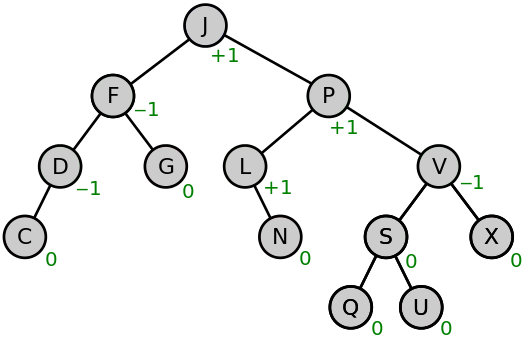
\includegraphics[width=8cm]{images/bal_tree_avl}  
  \end{center}
  \centerline{AVL дърво[1]}
  
  \end{frame}
  

\begin{frame}
\centerline{Въпроси?}
\end{frame}

\begin{frame}[fragile]
  \frametitle{Източници}
  
 [1]\href{https://en.wikipedia.org/wiki/AVL_tree}{Wikipedia:AVL Tree}
  
  \end{frame}



\end{document}

\begin{columns}[t]
  \begin{column}{0.55\textwidth}

  \end{column}
  \begin{column}{0.45\textwidth}

  \end{column}
\end{columns}
